\documentclass[17pt]{extarticle}

\title{Theatre Science}
\author{Williamson and Denton}
\date{February 2020}

\usepackage[margin=2cm,landscape]{geometry}

\usepackage[activate={true,nocompatibility},final,tracking=true,kerning=true,spacing=true,factor=1100,stretch=10,shrink=10]{microtype}
\microtypecontext{spacing=nonfrench}

\usepackage[T1]{fontenc}
\usepackage[utf8]{inputenc}

% Turn off page numbering
\pagenumbering{gobble}

% Baskerville font
\usepackage[osf]{Baskervaldx}

% For the images and resizebox
\usepackage{graphicx}

\usepackage{color}

\usepackage{pagecolor}
\pagecolor{black}
\color{white}

\begin{document}

\maketitle

\newpage

% Authority is constructed and contextual

\vspace*{1in}

{\Huge

\begin{center}

  Authority \\
  is constructed \\
  and contextual.

\end{center}

}

\newpage

% Definition of IL

{\Huge

  \begin{center}

``Information literacy is the set of integrated abilities encompassing the reflective discovery of information, the understanding of how information is produced and valued, and the use of information in creating new knowledge and participating ethically in communities of learning.''

    \end{center}

}

\newpage

\begin{center}
  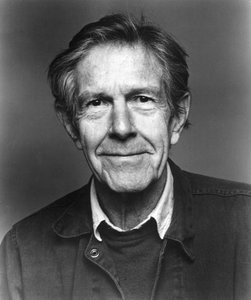
\includegraphics[height=7in]{images/john-cage-portrait.jpg}
\end{center}

\newpage

% Definition of IL

\vspace*{2in}
{\Huge

  \begin{center}

    Photo of Donald Gillies here.

    \end{center}

}

\newpage

\begin{center}
  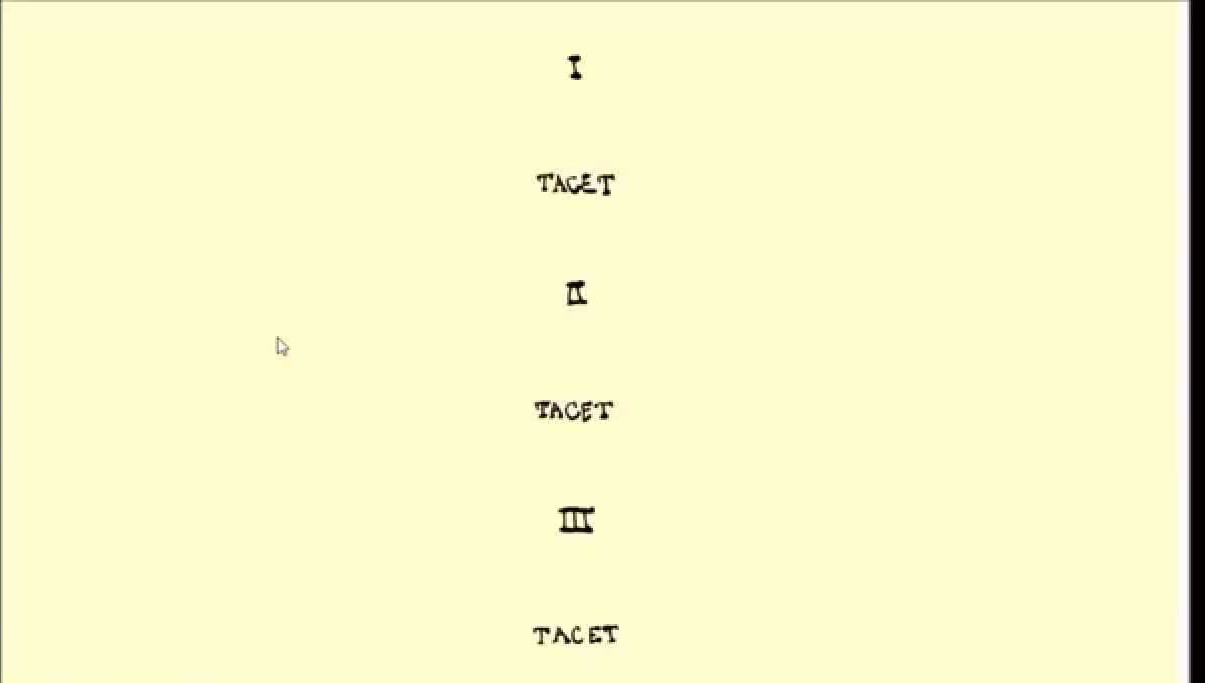
\includegraphics[height=6in]{images/433-score.jpg}
\end{center}

% Authority is constructed and contextual

\vspace*{1in}

{\Huge

\begin{center}

  Authority \\
  is constructed \\
  and contextual.

\end{center}

\newpage

% Definition of the frame.

\vspace*{1in}

{\LARGE

  \begin{center}

Information resources reflect their creators’ expertise and credibility, and are evaluated based on the information need and the context in which the information will be used. Authority is constructed in that various communities may recognize different types of authority. It is contextual in that the information need may help to determine the level of authority required.

\end{center}

}

\newpage

% Definition of the frame: sentence 1

\vspace*{1in}

{\LARGE

  \begin{center}

Information resources reflect their creators’ expertise and credibility, and are evaluated based on the information need and the context in which the information will be used. \textcolor{gray}{Authority is constructed in that various communities may recognize different types of authority. It is contextual in that the information need may help to determine the level of authority required.}

\end{center}

}

\newpage

% Definition of the frame: sentence 2

\vspace*{1in}

{\LARGE

  \begin{center}

\textcolor{gray}{Information resources reflect their creators’ expertise and credibility, and are evaluated based on the information need and the context in which the information will be used}. Authority is constructed in that various communities may recognize different types of authority. \textcolor{gray}{It is contextual in that the information need may help to determine the level of authority required.}

\end{center}

}

\end{document}
